\documentclass[tikz,border=10pt]{standalone}
\begin{document}

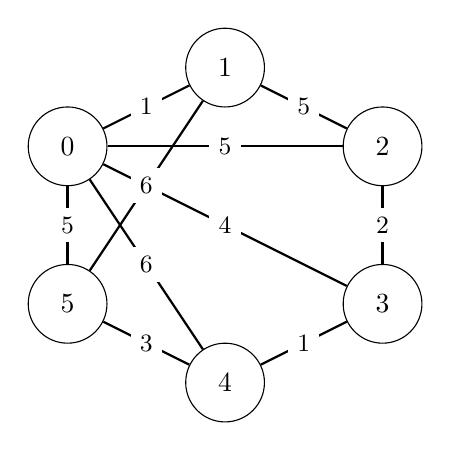
\begin{tikzpicture}[
  node/.style={circle, draw, minimum size=1cm},
  edge/.style={draw, thick},
  weight/.style={midway, fill=white, font=\small}
]

% Nodes
\node[node] (A) at (0, 3) {0};
\node[node] (B) at (2, 4) {1};
\node[node] (C) at (4, 3) {2};
\node[node] (D) at (4, 1) {3};
\node[node] (E) at (2, 0) {4};
\node[node] (F) at (0, 1) {5};

% Edges with weights
\draw[edge] (A) -- (B) node[weight] {1};
\draw[edge] (A) -- (C) node[weight] {5};
\draw[edge] (A) -- (D) node[weight] {4};
\draw[edge] (A) -- (E) node[weight] {6};
\draw[edge] (A) -- (F) node[weight] {5};

\draw[edge] (B) -- (C) node[weight] {5};
\draw[edge] (B) -- (F) node[weight] {6};

\draw[edge] (C) -- (D) node[weight] {2};

\draw[edge] (D) -- (E) node[weight] {1};

\draw[edge] (E) -- (F) node[weight] {3};

\end{tikzpicture}

\end{document}
